\chapter{Methodology}
The introduction outlined the purpose of the project: to create a framework for accelerated development of learning models for the reconstruction of action models, and a proof of concept implementation to display the effectiveness of such a framework. We defined a set of constraints which the framework must satisfy in order to be a viable tool for research. In this chapter we will discuss the problems taken into account before development. We will also provide a detailed account of development and review implementation issues we faced.

In the first section we will discuss the scope of the problem we are attempting to tackle. Attempting to tackle too many features will lead to feature creep (excessive addition of features leads to difficulty in use and development). This is especially important when cumulative development time is limited. A well defined scope will also ensure that targets are satisfied and the road map for future development is much easier to design.

In the next section we will discuss the baseline for evaluation. We are defining the minimum use-case of the framework that will demonstrate its capability in a given scenario. We discuss the advantages and limitation of our baseline and an outline of general issues that needed to be answered before implementation. We also need to define the output format of results and their credibility.

Finally we will review our analysis in itself. We will discuss the methods we took into consideration for the interpretation of our results, and provide a review of the relevance of our work in a quickly evolving field.
\newpage


\section{Problem Scope}
Prior to tackling a problem, a scope needs to be defined. This includes identifying what tasks have already been solved and which have not, as well as outlining the relative difficulty of each task. This allows us to identify which issues require more resources and plan accordingly. We outlined in our introduction the objectives we want our framework to satisfy. In this section we will leverage our knowledge of existing work \ref{background:Existing Work} to define the scope for each objective, estimated work and any compromises leading to eventual limitations.

\subsection{Environment and accessibility}
In this section we will specify our development pipeline, its product, advantages and limitations. The tools and frameworks used for development can make or break a project. We already stated that development would be done in python, however we did not define how the average user could take advantage of the framework we have developed. Given that the scale is relatively small, we decided to set up a minimalist pipeline in order to conform to best practices.

As with any project version control is required, our experience is with Git hence we chose GitHub (a popular platform for managing git repositories) to host our work and manage development. To begin with we decided to stick with tools provided by GitHub as adding third-party building and deployment frameworks such as Jenkins would be unnecessary at this stage. Bellow is a figure displaying our development pipeline at this stage we will go over it in detail.

\begin{figure}[h]
    \centering
    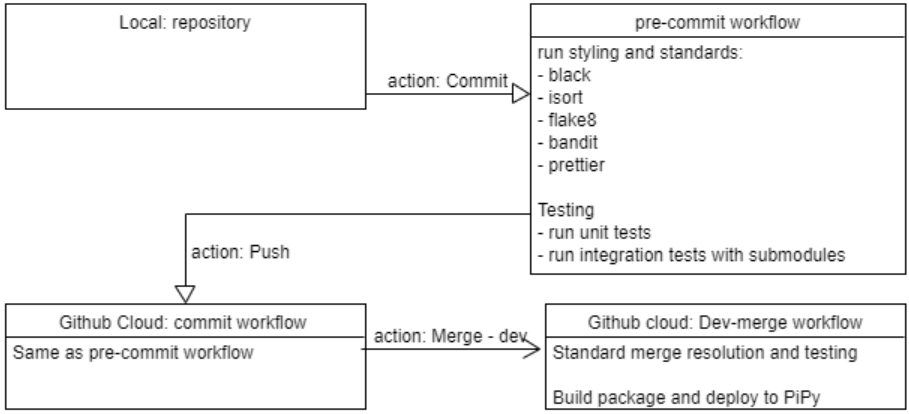
\includegraphics[width=\linewidth]{images/architecture/git-flow}
    \caption{development workflow in git.}
    \label{fig:git-flow}
\end{figure}
\newpage
We followed the agile development process focusing on delivering incrementally and ensuring code is tested and well maintained. To support this we set up a delivery pipeline as seen in figure \ref{fig:git-flow}. We used common tools to ensure python development standards were followed. Black is a code formatting engine ensuring that code looks the same regardless of the programmer. Black enforces a code style transparently and is used by a large number of open source projects and communities. Isort ensures that imports are sorted correctly, preventing Houdini style occurrences of imports mid-way through a file. Flake8 ensures conformance with the PEP8 standard, this includes preventing occurrences of unused imports, and common python programming malpractice such as using\(==\) instead of \(is\) in certain situations. Although most likely unnecessary we decided to include Bandit, a tool designed to find common security issues in python as well. Finally we use prettier to format code automatically in order to make our lives easier when conforming to bandit styling, this allows developers to program in their desired environment without worrying about maintaining a strict style required by black.

For testing we used standard python unit tests, and added hooks to GitHub on a merge action to ensure all tests are passing before a new version of the package is pushed to PiPy. We followed the TDD style of development when working on main modules in order to ensure functionality is stable and works as expected. When modules interact or become more complex this stave a lot of time. The final stage of our workflow is the delivery of a package to any potential users. We decided to use PiPy a popular hosting platform for delivery of pip packages (the most standard library distribution framework in python).

This pipeline we determined is the minimum setup for any viable project aiming for wider use and future development. The advantages of this pipeline are that it is relatively simple hence little to no maintenance is required once everything is set up. This ensures that not time is wasted on unnecessary dev-ops. Having such a pipeline also ensures that agile development can be practiced effectively as we do not have to worry about large integration tests as the process is very iterative. This pipeline also provides stability which is often lacking when performing research as code often breaks and new approaches are added. There are limitations however, one such limitation is the lack of different environments such as development staging and live, although we determined this is unnecessary at this stage and is easily implemented int he future. Another limitation is the lack of testing across multiple environments and versions, we assumed that libraries must be up to date, which may cause issues as backward-compatibility may be important in some use-cases, especially when integrating with older libraries or projects.
\newpage

\subsection{Scope of objectives}
In this section we will review our objectives for the framework and ground them in reality. We need to analyse what features or functionalities are indispensable and which are of less importance. The purpose of this is to ensure that we do not tackle unnecessary problems that can be resolved by simply scaling the project, i.e. a module may not be viable without a core feature, but will be fine without all non-essential features being implemented to date. Take a calculator for example, each calculator has a given complexity or ability to compute problems at different scales, however if you remove a core module of the calculator (such as the ability to process input from the user) then no matter which calculator you choose none will be useful. This is the challenge when building an MVP (minimum viable product).

Our first objective is support for parsing various domain languages to a python standard. We have explored in our related work section that previous work has been attempted, but with little success meaning it will not be viable for our platform. for this reason we have decided to build a parser and translator to python from scratch. As PDDL has evolved we have decided to start with the most basic version and add to it iteratively, this way if we don't complete support for a higher version, we will still have a lower version we can rely on. We are targeting PDDL 2.2 with full test coverage on both the parser, transformer and python representation. We decided to go with PDDL due to the problems we were already working on and it's popularity amongst the planning community. Secondly we want to ensure that we provide an interface layer so that other languages may be supported in the future. If time permits it we may interface a second language if an existing parser exists.

\begin{figure}[h]
    \centering
    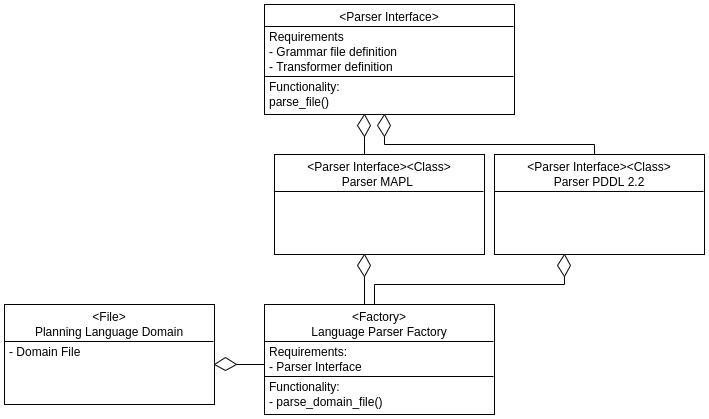
\includegraphics[width=1\linewidth]{images/architecture/parser_uml}
    \caption{Basic parser functionality requirement UML.}
    \label{fig:parser-uml}
\end{figure}
\newpage
Our second objective is to support generation of training data. Here we face our first issue. Training data for planning comes in many formats hence we must define an acceptable standard which is flexible enough to support current development of planning algorithms and maximises existing data generation techniques. We decided that we do not need to place much focus on actual data generation scripts as these are widely available and provide required data-sets in various formats, sizes and languages. We will instead focus on making it as simple as possible to add any existing script for data generation and integrating it with our platform for users to take advantage of. Integration will also involve standardising output format of such scripts. We will be adding several widely available scripts for initial use. This task is not very complex as a lot already exists.
\begin{figure}[h]
    \centering
    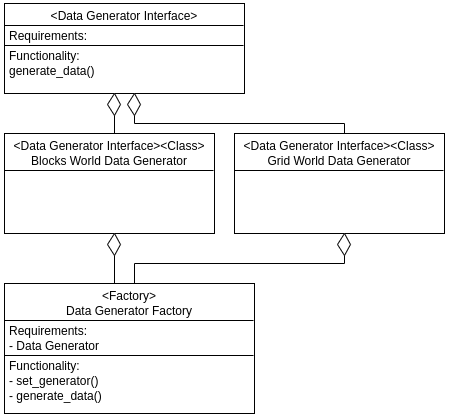
\includegraphics[width=0.7\linewidth]{images/architecture/data_generator_uml}
    \caption{Basic data generation requirement UML.}
    \label{fig:data-generator-uml}
\end{figure}


The third objective is "Simplified implementation of learning models".
This was set in order to make sure that when new users attempt to extend or add new learning models, the rules and requirements to do so are clear and simple to follow.
Hence our scope for this objective is to provide an implementation of an existing learning model (Markov Logic Networks) as well as the abstract classes, to ensure future expandability is guaranteed. We will compare the integration time of the exisitng learning model with our framework with the work done by other papers of similar complexity to generate results.
We aim to make sure that our implementation is decoupled from the framework as a showcase of how one might use with the framework.
We will not be adding multiple learning models as such models compatible with python are not widely available for the precise reason that research code is often missing or broken, hence integrating an existing implementation is an intensive process if one is not familiar with the work.
We have included the architecture diagram displaying how a custome learning model would be integrated \ref{fig:learning-model-uml}
\begin{figure}[h]
    \centering
    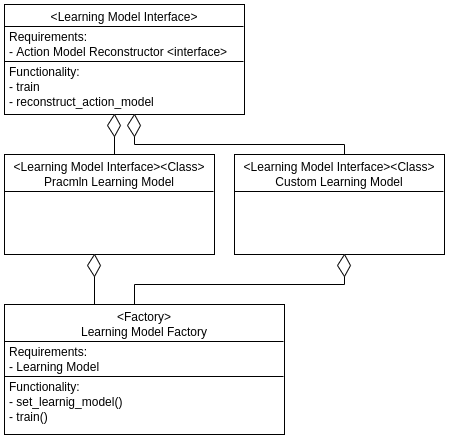
\includegraphics[width=0.7\linewidth]{images/architecture/learning_model_uml}
    \caption{Basic learning model integration UML.}
    \label{fig:learning-model-uml}
\end{figure}

The fourth objective involves the implementation of extendable modules for conversion of training output to a standard action model. We came to the conclusion that these modules are specific to the learning model output hence methods we use for conversion will be proprietary. However our objective is to make it possible for different learning techniques that have the same output to be able to share an action model reconstruction module. This means each module must make it's input data clear to potential users, Python supports typing and we can use documentation to enable such work. We made the decision to provide two action model reconstruction modules in order to demonstrate the use cases these satisfy. A generated action model must be compatible with our simulation module hence for now output is restricted to the only supported language PDDL.
\begin{figure}[h]
    \centering
    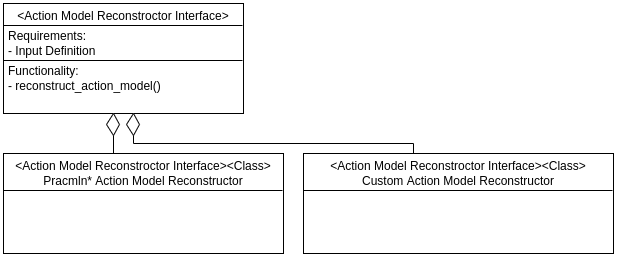
\includegraphics[width=0.7\linewidth]{images/architecture/action_model_reconstructor_uml}
    \caption{Basic action model reconstructor implementation UML.}
    \label{fig:action-model-reconstructor-uml}
\end{figure}
\newpage
The fifth objective is developing a testing framework for learned action models. We will create a python based simulation module taking the learned action models as input and some test data for simulation of the reconstructed action models. We will base the simulator on rules taken from PDDL 2.2 planners. Our objective for the simulator is to generate data and compare data between differently generated action models. We will make such a simulator as modular as possible allowing for simulators written in other languages to be used as well if they exist. Work on simulation has been done, however we deem it important to provide our own as the work is necessary either way if we are translating a planning definition language into python.
\begin{figure}[h]
    \centering
    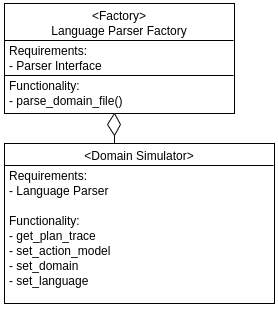
\includegraphics[width=0.4\linewidth]{images/architecture/domain_simulator}
    \caption{Basic action model reconstructor implementation UML.}
    \label{fig:domain-simulator-uml}
\end{figure}

The figures we have presented provide the minimum scope we wish to satisfy for each module, hence they are to be taken as an indicator rather than a full fledged design implementation. We have not provided the full interaction between modules or their full design specification as that will only complicate the ideas we are communicating.

The sixth and final objective is User-friendly and modular adoption of the framework.
For this objective we have decided to follow the same approach that most model ML libraries have adopted.
The idea is to release a python package similar to one such as Tensorflow, and expose each of our modules for the user's benefit.
The reasoning behind this approach is that users will be able to use our framework for projects that have little to do with action model reconstruction.
As we support parsing PDDL and simulating domains, tasks such as writing a PDDL solver or integrating with an ML library can be done directly in python without worrying about interpreting the domain files, this is similar to how pandas allows users to load a CSV file into a DataFrame object, we provide the user with the ability to load a Domain or Problem file into their respective data structures and apply operations over them.
The reasoning behind this approach is that if users determine that these modules are helpful, they will report issues and contribute towards their development, keeping these modules separate ensures that each user can cater the platform and their contribution to their requirements.

A sample project similar to a Jupyter project will be included in the repository, using each module to load a sample domain, generate a dataset of problem states and solutions, and finally train and evaluate a model.
This will be an initial entry point and documentation for any user willing to try using the framework.


\newpage
% 
% sections: Problem Scope


\section{Minimum use-case}
% In the next section we will discuss the baseline for evaluation. We are defining the minimum use-case of the framework that will demonstrate its capability in a given scenario. 

\subsection{Defining baseline objectives}
In order to test the viability of our framework we must define a sample implementation that reflects a vertical slice including all functionality available.
This use-case must reflect the functionality that a student or researcher in the field would require when working on planning problems.
This will provide enough evidence to compare the difference in workload between using our framework and proceeding without. Our aims are as follows:
\begin{enumerate}
    \item Design and generate a database for training a Markov Logic Network, leveraging available domains, problem generators and solvers.
    \item Train a Markov Logic Network.
    \item Evaluate the accuracy of the network given different noise levels.
    \item Reconstruct action models from the trained network.
    \item Compare the reconstructed model with their original counterparts
\end{enumerate}
We can argue that the above steps are common when working on any learning model, most research time may be spent on developing the model itself, however evaluation and analysis is also imperative as new methods need to be compared with existing ones. These steps are useful because they will demonstrate the effect of having a support framework when it comes to menial tasks such as data collection.

The limitations of such a baseline is that it does not expose the framework to enough use cases, it is difficult to gauge the impact of what we have developed based on only one sample implementation. This will only be resolved after wider adoption. As users adopt the framework, unseen issues in the architecture will surface and have the opportunity to be resolved.



% TODO: Formal definition of data we wish to collect

% We discuss the advantages and limitation of our baseline and an outline of general issues that needed to be answered before implementation. We also need to define the output format of results and their credibility. 

\newpage
\section{Analysis}
In this section we define the scope and format of data which we would like to collect to ensure that we can draw satisfactory conclusions from it.
This includes data we require for ensuring the implementation of our learning algorithm is viable, and the data required to gauge how much work went into integration with the framework and how useful our resulting implementation would be for the average user in comparison to other commonly existing implementations.

%framework metrics: reliability, maintainability, testability, portability, reusability
% user metrics: adoption friction, learning curve, development complexity

% \subsection{Defining our use-case}
